\documentclass[english]{scrartcl}



\usepackage[maxbibnames=9, backend=biber]{biblatex}
\bibliography{papers}
\bibliography{references}


%%% === Fonts ==============================================
\usepackage{lmodern}
\usepackage{MnSymbol}
\usepackage{bold-extra} %% bold type writer font % [cmbtt]
\usepackage{relsize}    %% \smaller
\usepackage[svgnames,table]{xcolor}

%% === Language ===========================================
\usepackage{babel}
\usepackage{csquotes}
\usepackage{fontspec}
\newcommand{\q}[1]{\enquote{#1}}
\MakeOuterQuote{"}

%% === Bibliography =======================================
\usepackage[backend=biber]{biblatex}

%% === Code Listings ======================================
\usepackage{listings}
\lstset{captionpos=b, xleftmargin=1cm}
\lstset{basicstyle=\small\ttfamily, showstringspaces=false, columns=flexible, keepspaces=true}
\lstset{tabsize=2, gobble=2}
%\lstset{upquote=true}
%% Linebreaks
%\lstset{prebreak=\raisebox{0ex}[0ex][0ex]
%        {\ensuremath{\rhookswarrow}}}
\lstset{postbreak=\raisebox{0ex}[0ex][0ex]{\ensuremath{\rcurvearrowse\space}}}
\lstset{breaklines=true, breakatwhitespace=true}
%% Line Numbers
\newcommand{\lstnumberstyle}[1]{\tiny\emptyaccsupp{#1}}
\lstset{numbers=left, numberstyle=\lstnumberstyle, numbersep=5pt,
		numberfirstline=false, firstnumber=auto, stepnumber=5}
\lstset{language=Java}
\lstset{escapeinside={(*@}{@*)}}
\lstdefinestyle{EclipseStyle}{
	keywordstyle=\bfseries\color{Purple},
	stringstyle=\color{Blue},
	commentstyle=\color{Gray},
}
\lstdefinestyle{NetBeansStyle}{
	keywordstyle=\bfseries\color{Blue},
	stringstyle=\color{DarkOrange},
	commentstyle=\color{Gray},
}
\lstdefinestyle{BWStyle}{
	keywordstyle=\bfseries,
	stringstyle=\color{DimGray},
	commentstyle=\textsl,
}
\lstset{style=BWStyle}

\lstdefinelanguage{algorithm}{
	keywords={function, for, do, if, then, else, return, in_, is_a, or, and},
	morecomment=[l]{'},
	morecomment=[s]{/*}{*/},
	morestring=[b]",
	sensitive=true,
}
\lstdefinelanguage{HanaSQL}[]{SQL}{
	morekeywords={replace,string,if,daysbetween,secondsbetween,weekday,adddays,addseconds,double},
	moredelim=**[is][\slshape]{^}{^},
	moredelim=**[is][\bfseries]{§}{§},
}
\lstdefinelanguage{Inline}{
	moredelim=**[is][\slshape]{^}{^},
	moredelim=**[is][\bfseries]{§}{§},
}

\newcommand{\lineref}[2]{\hyperref[#1]{line~\ref*{#1:#2}}}
\newcommand{\linerefn}[2]{\hyperref[#1]{line~#2}}

%% === More Tools =========================================
\usepackage{accsupp}
\newcommand\emptyaccsupp[1]{\BeginAccSupp{ActualText={}}#1\EndAccSupp{}}
\usepackage{ctable}

%% === Links and References ===============================
\usepackage{hyperref}
\usepackage[nameinlink, noabbrev]{cleveref}	%% \cref commands
\usepackage[all]{hypcap}
\hypersetup{
    hidelinks,
    plainpages=false,			%
    bookmarksopen=true,
    bookmarksnumbered=true,
}

\usepackage{todonotes}

\title{Omniscient Debugging in Enterprise Applications}
\subtitle{Working Title}
\author{Arian Treffer}

\begin{document}

\maketitle

\begin{abstract}
Developers spend between 40 and 60 percent of their time working on defects.
A lot of that time is spend in the debugger, searching for the cause of an observed problem.
While debugging, the developer's attention is divided between multiple tasks, which fall into two categories:
first, understanding the program at different levels of abstraction and second, operating the debugger and other related tools.
Attention spent in the first category will directly let the developer progress towards her goal, whereas the second category represents a necessary overhead that should be kept to a minimum.
Unfortunately, the mental overhead imposed by regular debugging tools is often quite large.
Debuggers work with very low and technical concepts, such as variables and instructions.
The mapping to higher conceptual levels is left to the developer.
Furthermore, debuggers are unforgiving: a step to far and the entire debug session has to be restarted.
Thus, the developer is forced to step forward with utmost care, which requires a level of attention that makes it difficult to think about the actual problem simultaneously.
When a mistake is eventually made, even in a best-case scenario restarting the debug session takes at least a couple of seconds, enough time to lose an important train of thought.

In our work, we combine existing concepts of omniscient debugging and object-centric debugging to create a Java debugger that allows the effortless navigation of program executions. 
Using a postmortem approach, our debugger works on recorded execution traces and is able to recreate the program state from any point in time.
This way, the developer can step not only forwards, but also backwards through the execution -- in fact, any jump through time is instantly possible.
Additionally, we devised a new configurable algorithm for dynamic slicing that fits the interactive nature of the debugging workflow.
In sum, we were able to create a debugging toolchain that helps the developer to investigate complex problems without diverting her attention to tool operation.

Large and complex applications also often use a database to handle complex operations on large amounts of data.
While most modern databases allow to attach a debugger to queries or scripts, the general tool support for understanding complex programs in databases is rather poor compared to that of popular object-oriented languages.

To accommodate the demand for better debugging tools in database programs, we transferred our research findings to SQL Script.
We developed a method to leverage the mix of imperative control flow and declarative SQL statements in SQL Script. 
This allowed us to created an omniscient debugger which is much more efficient with large amounts of data than previous solutions for object-oriented languages.
Furthermore, we adapted our dynamic slicing algorithm to the increased complexity by implementing different levels of accuracy.
This way, the debugger can quickly present an approximation of the slice.
The developer can then choose for which parts an exact slice is to be computed.
We can show that our algorithms are fast enough even for complex scripts and large amounts of data.
Thus, our concepts are fit to to be integrated into database application development tools and can provide state-of-the-art debugging techniques to enterprise application developers.

\end{abstract}

\section{Introduction}

\subsection{Motivation}
Why debugging is important and its shortcomings.\\
better tools improve efficiency

\subsection{Research Questions}
How can debugging be improved to reduce the time needed to find a bug?\\
1) Which operations are needed for the efficient navigation of a program execution?\\
2) Which questions developers ask can be answered automatically?\\
3) How can programs handling large amounts of data be debugged and analyzed efficiently?\\

\subsection{Outline and Contributions}

1) Unification of omniscient and object-centric debugging\\
2) Interactive dynamic slicing for iterative refinement of problem space\\
3) SQL Script adaption of previous concepts\\

\section{Related Work and Background}

\subsection{The Snake in the Grass}
Omniscient debugging, debugging related tools

\subsection{Programmers Think in Slices}
static and dynamic slicing, other dynamic analysis tools\\
problem with existing algorithms: too slow, usefulness of results vary

\section{Java Omniscient Debugger}
Motivation: why new tool?
Existing Java ODB not in IDE, object model requires much memory, not optimized for dynamic analysis

\subsection{Efficient Tracing of Java Applications}
How the Java Agent works, how to «trace everything», evaluation of overhead.

\subsection{Modeling the execution trace}

Debuggers are a special kind of runtime analysis tools.
Generally, there are two ways to implement a runtime analysis.

A live analysis evaluates the program as it is executed; as soon as, or even before, the program terminated, the result of the analysis is available.
Common debuggers typically fall into this category.

A post-mortem analysis first records aspects of the programs execution and then analyses the recorded data.
Sometimes, this approach has the advantage that multiple analyses may be run iteratively, without having to re-execute the program.
This disadvantage of this approach is that, depending on the granularity of the recorded data, it requires much more memory.

Backwards debuggers can be implement with both the live and the post-mortem approach.
In the scenario described above, where the debug session begins at the occurrence of a failure, it does not make much of a difference.
In other use cases, however, the look-ahead that is possible with the post-mortem approach can make the difference between a backwards and an omniscient debugger.

Many strategies have been proposed to reduce the amount of data that has to be captured to allow a replay of the execution.
However, since we aim for an omniscient approach, we will record almost everything, including method calls and returns, exceptions, and variable and field accesses.

Figure \ref{fig:model} shows how the execution trace is modeled.
The trace model consists of two parts.

%\afterpage{

\begin{figure}[t]
\centering
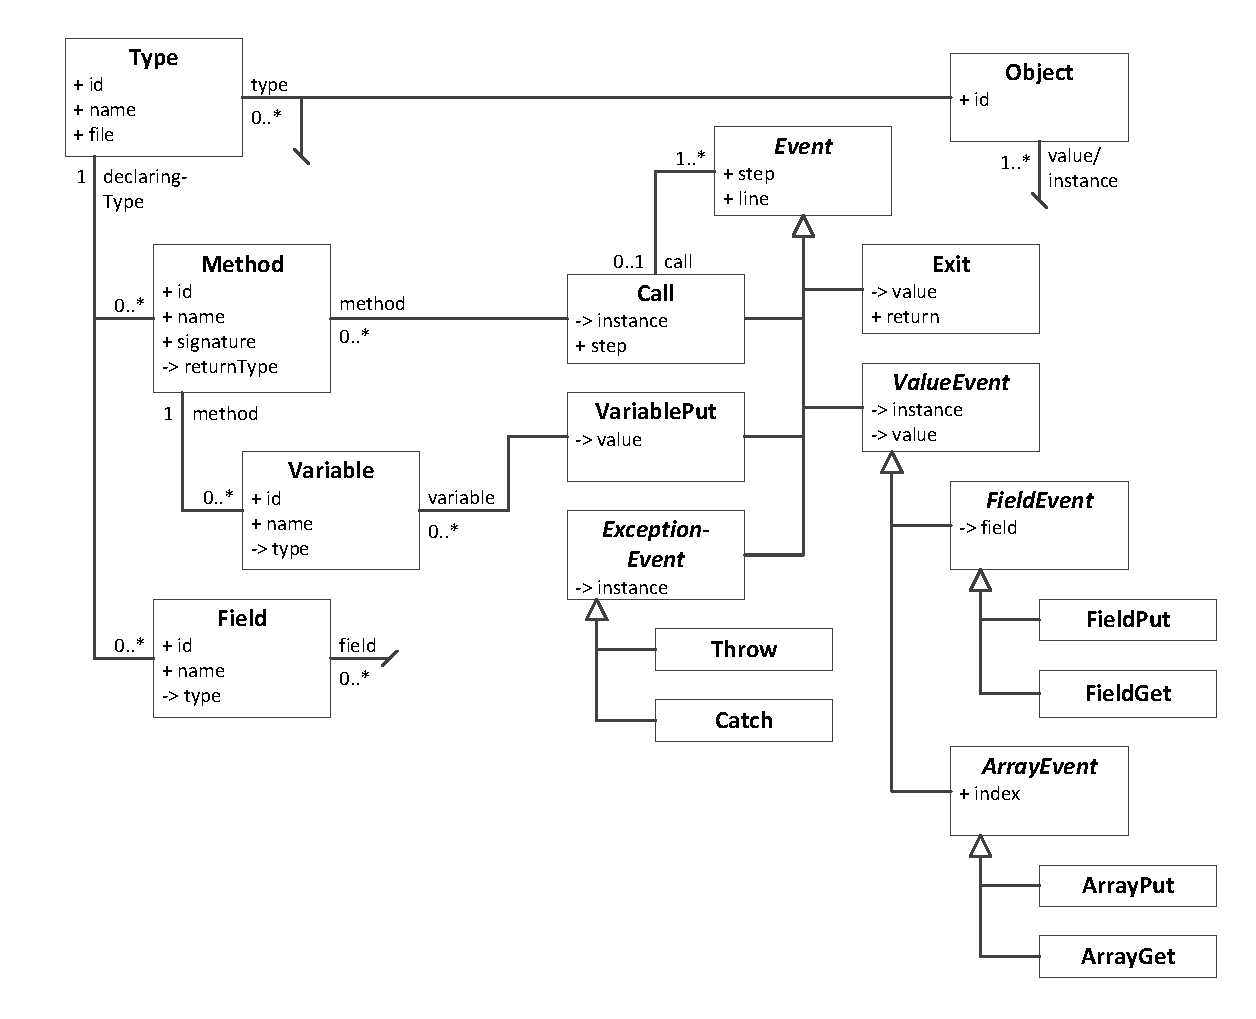
\includegraphics[width=.7\textwidth, clip, trim=5mm 5mm 5mm 5mm]{img/model.pdf}
\caption{Trace Model}
\label{fig:model}
\end{figure}

%\clearpage
%}

The static part describes the application's code on a high level.
Classes, fields, methods, and variables are represented with enough properties to find them in the code base, so that they can be referenced from the actual trace data.

The dynamic part identifies all objects that occurred during the execution and contains events that happened with these objects.
Every event is identified and ordered by a step number and contained in a parent method call (except for the root call).

The program flow is described with call events, which reference the method and the instance on which it was called, and their respective exit events which provide the result value and indicate whether the method terminated via return or exception.
Additional program flow is provided by exception throw and catch events.

Value events indicate changes and side-effects of the program state.
Represented are field and array reads and writes, as well as variable changes.
This way, the state of an object or the variable assignments at a certain point in time can be easily derived from the latest respective set events.

Based on this model, it is possible to develop a debugger that can revert and replay the execution of a program and provide snapshots of the state at any point in time.

\todo[inline]{evaluation of memory usage}

\subsection{Back to the IDE}

As described above, a recurring task is to find the source of a value.
It seems obvious how a backwards debugger can improve the time required to find the source of an error.

Restarting the debug session becomes virtually unnecessary.
Once an error is identified, the developer can step backwards to its source.
If a method call is stepped over by accident (in either direction), the operation can be easily reverted.

Nevertheless, this may still require stepping (backwards) through large parts of the application.
An omniscient debugger, on the other hand, immediately knows where the value was set.

\begin{figure}[ht]
\centering
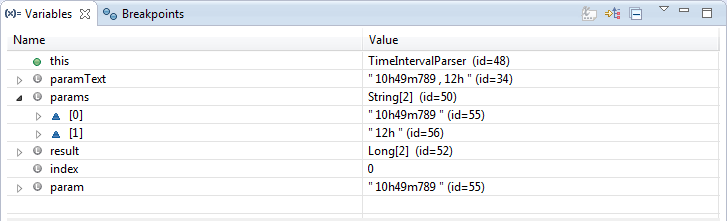
\includegraphics[width=.8\textwidth]{img/variables.png}
\caption{Variables View in Eclipse}
\label{fig:variables}
\end{figure}

Figure \ref{fig:variables} shows the variable view of Eclipse's debugging perspective, which is typically used to spot erroneous values.
With the omniscient debugger extension, the developer can directly jump back in time to the assignment of a value simply by double clicking it.
This changes the debugging process as follows:

The developer finds the value and double-clicks to jump to its source.
She finds that the value is build from three other values, using a formula that seems to be correct.
However, she is not sure which of the input values is erroneous.
Thus, she bookmarks the current point-in-time and begins to investigate the first value, again by double-clicking it.

Once she stepped around through the value's creation, she is certain that this value is valid and uses the bookmark to return \emph{back to the future}.
Then she begins to investigate the second value.
When she realizes that it is invalid, this process is repeated until the fault is reached.

As the example shows, another important task is to determine whether a value is valid by examining how it is produced.
Here, the omniscient debugger can assist in multiple ways.

Firstly, instead of showing just the current stack trace, the omniscient debugger can provide a tree of previous and subsequent invocations (cf.\cref{fig:tree}).
Especially after jumping backwards, the developer may have to regain orientation, where this additional context can be helpful.

\begin{figure}[ht]
\centering
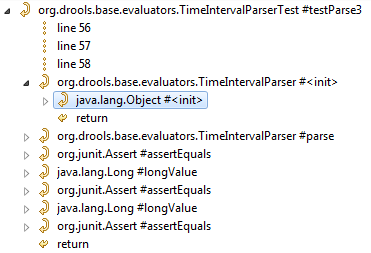
\includegraphics[width=.55\textwidth]{img/tree.png}
\caption{Call Tree}
\label{fig:tree}
\end{figure}

Secondly, the debugger can show the history of a variable, or even an entire object (cf.\cref{fig:history}).
Mostly, this is helpful when a value is created in a loop or if an object is changed in multiple, different parts of the application over a longer stretch of time.

\begin{figure}[ht]
\centering
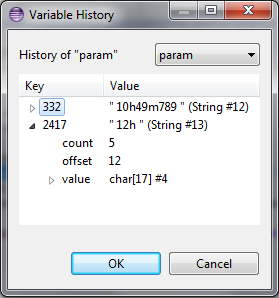
\includegraphics[width=.4\textwidth]{img/history.png}
\caption{Variable History}
\label{fig:history}
\end{figure}

Finally, the debugger knows whether a given value is used again or at all.
By greying out variables and fields that are not accessed again (at least not before their values are changed), the program state that has to be examined by the developer is effectively reduced.

\section{Object-centric Debugging}
Scenario: developer is concerned with particular object\\

\begin{figure}[ht]
\centering
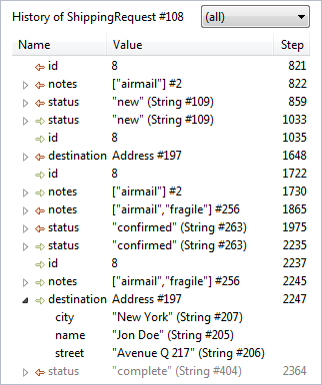
\includegraphics[width=.4\textwidth]{img/objecthistory.png}
\caption{Processing a shipping request, shown as a sequence of field accesses}
\label{fig:history}
\end{figure}

\subsection{Aspects of Interest}
history of object, side effects, method invocations\\
how typical programmer questions can be easily answered this way\\
where this information is found in the trace

\subsection{Complementing the Variables View}
The object/history view as an inviting, low-barrier entry point.\\
From there, trick the developer into object-centric debugging.\\
Performance considerations.

\section{Interactive Dynamic Slicing}
Motivation: developer looking for relevant code in a large execution

why slicing is good but existing algorithms (though very advanced) have usability problem\\


Dynamic analysis can provide much more concrete insights into the execution of a program than its static counterpart.
Where static analysis has to apply complex algorithms to determine, for instance, if two variables can reference the same object or which methods a virtual method call might invoke, dynamic analysis can rely on actual data.
Assuming that the analyzed execution was representative, insights may even be generalized for the whole program.
Nevertheless, dynamic analysis cannot survive on its own~\cite{binkley_theoretical_2006}.

There are two approaches to dynamic analysis.
On the one hand, the program can be analyzed statically before execution to insert specific trace statements that will retrieve relevant information~\cite{ko_debugging_2008}.
On the other hand, the whole execution can be recorded.
In this case, the output usually is a sequence of events where many of the semantics of the code have been lost.
For instance, knowing the byte-code that produced an event does not tell whether it was part of a branching conditional, a loop, or a method call argument.
Thus, some form of static analysis is required to map recorded events to their meaning in the source code.
Furthermore, if more than trivial questions about the execution have to be answered, additional static analysis is required to detect relations between events that can be subject of a subsequent dynamic analysis.

A typical example for a combination of static and dynamic analysis methods is slicing, a techniques that allows to remove statements from a program to help the developer to focus on the causal dependencies of a specific part of the program.
According to Weiser~\cite{weiser_programmers_1982}, a (static) slice $S$ is a subset of the statements of a program $P$ on a slicing criterion $C$, so that for any input $I$, $S$ and $P$ produce state trajectories equivalent with respect to $C$.
A typical example for a slicing criterion would be a variable in a given line.
Then, all statements that can never impact the value of that variable can be removed from the slice.
Dynamic slices are defined similarly, but have to produce the equivalent state trajectories only for specific inputs~\cite{korel_dynamic_1990}.

It has been shown that slicing represents how programmers naturally think about problems in programming~\cite{weiser_programmers_1982} and has many applications, including, but not limited to, debugging~\cite{agrawal_debugging_1993} and program comprehension~\cite{de_lucia_program_2001}.

We used Soot to provide the foundations of a dynamic analysis.
By generating specialized intraprocedural dependency graphs and matching them against events from an execution trace in an omniscient debugger, we were able to produce debuggable dynamic slices.

Soot allowed us to easily create dependency graphs that track different types of dependencies between statements.
Compared to previous approaches to dynamic slicing, this gives us more control when choosing which statements to include in a slice.
In particular, based on the user's needs, our approach can generate different slices for the same criterion and input.
By focusing the slicing on events instead of statements, we increased the precision of the slices even more.

\subsection{Configurable Dependency Algorithm}

As shown in \autoref{lst:test}, the test validates that a string of comma-separated time intervals can be parsed into an array of long values, with each value being the respective time in milliseconds.
The actual parse method, shown in \autoref{lst:parse}, splits the string at each comma and parses each substring individually.

\begin{lstlisting}[firstnumber=54,float,caption={A test in TimeIntervalParserTest.java},stepnumber=2,label=lst:test]
    @Test
    public void testParse3() {
        String input = " 10h49m789 , 12h ";
        long expected1 = 10 * 3600000 + 49 * 60000 + 789;
        long expected2 = 12 * 3600000;
        Long[] result = new TimeIntervalParser().parse( input );
        assertEquals( 2, result.length );
        assertEquals( expected1, result[0].longValue() );
        assertEquals( expected2, result[1].longValue() );
    }
\end{lstlisting}

\begin{lstlisting}[firstnumber=34,float,caption={The method under test, implemented in TimeIntervalParser.java},stepnumber=2,label=lst:parse]
    public Long[] parse(String paramText) {
        if ( paramText == null || paramText.trim().length() == 0 ) {
            return new Long[0];
        }
        String[] params = paramText.split( "," );
        Long[] result = new Long[params.length];
        int index = 0;
        for ( String param : params ) {
            String trimmed = param.trim();
            if ( trimmed.length() > 0 ) {
                result[index++] = TimeUtils.parseTimeString( param );
            } else {
                throw new RuntimeDroolsException( "Empty parameters not allowed in: [" + paramText + "]" );
            }
        }
        return result;
    }
\end{lstlisting}

A typical scenario could consist of a developer who is only interested in particular values of the array.
For instance, the developer might wonder how the value that is passed to the second assert, in \linerefn{lst:test}{62}, is computed.

In this particular example, it would be easy for the developer to set a breakpoint in \linerefn{lst:test}{44}, skip the first iteration, and then step into the second invocation of \verb+parseTimeString+.
However, developers often find themselves in similar situations where finding the right invocation is not as simple, possibly for one of the following reasons:
The developer might not be familiar enough with the code to find the right location for setting a breakpoint, there might be too many iterations to make skipping them manually feasible, or the actual iteration is unknown because elements are reordered or removed later on.

In other scenarios, the developer may not know the actual path through the program because of complex branching, virtual method calls, or exceptions.
In these cases, it might even be more interesting to get an overview of the path than having to step through the application manually.

\begin{figure}
\centering
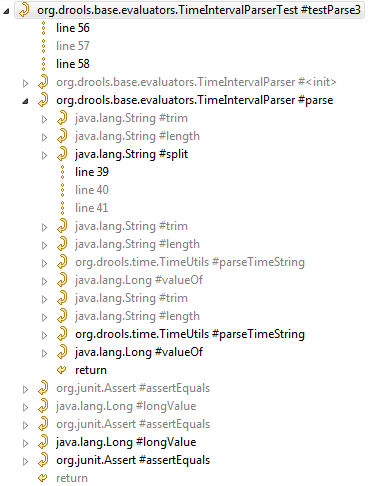
\includegraphics[width=.75\linewidth]{img/calltree}
\caption{A tree of method invocations. Gray nodes are not part of the current slice.}
\label{fig:calltree}
\end{figure}

For our particular example, the developer would right-click the second \verb+assertEquals+ invocation and chose ``slice'' from the context menu.
Then, the slice for that invocation is computed and irrelevant operations are removed from the execution, i.e., they are displayed in gray in the call tree, as shown in \autoref{fig:calltree}, and are no longer accessible via stepping.

\subsection{On-the-fly Slice Computation}
%Our slicing algorithm, now adapted to allow incremental modifications.


Typically, static and dynamic slicing algorithms focus on finding statements belonging to a slice.
However, in many cases statements are executed multiple times in a single program run and not all executions are relevant for the slice.
Therefore, our algorithm focuses on state-changing events, i.e., actual executions of statements, instead of the statements themselves.

On the highest level, our algorithm to compute a dynamic slice works as follows:
The output of the algorithm will be a sorted set of events.
The target event, i.e., the event for which the slice was requested, is added to both the result set and a queue of unprocessed events.
Then, until the queue is empty, an event is polled and its dependency events are determined as follows:

%Firstly, the event is mapped to a unit of a \verb+SootMethod+.
Firstly, the event is mapped to a statement in the code.
Secondly, Soot is used to obtain a static dependency graph for that method (the graph is cached for reuse).
Thirdly, the statement is looked-up in the graph and candidate dependency statements are mapped back to events.

Each dependency event that is not yet part of the result set is added to both the result and the queue.
Finally, the result set is returned.

\begin{figure*}[t]
\centering
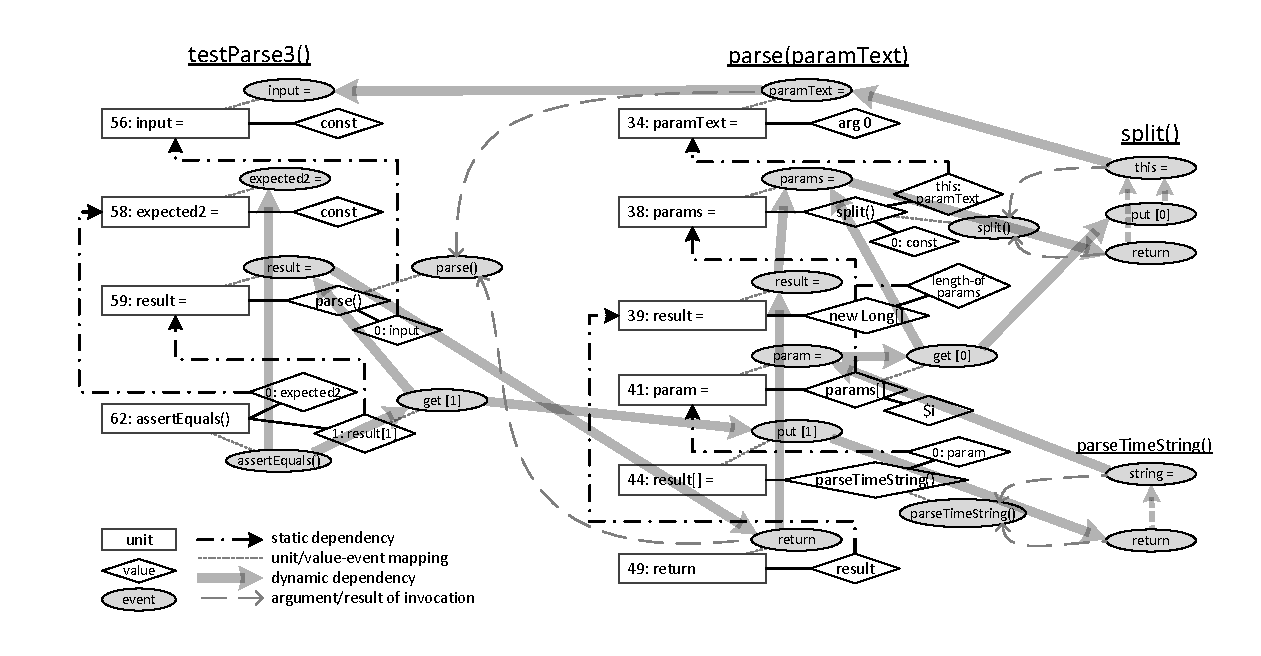
\includegraphics[width=.99\linewidth, clip, trim=12mm 7mm 8mm 7mm]{img/graph}
\caption{A dynamic dependency graph of trace events, on top of static dependency graphs derived with Soot. For brevity, not all Soot units are shown, the boxing of long values has been omitted, and ``split'' and ``parseTimeString'' are summarized.}
\label{fig:graph}
\end{figure*}

\subsubsection{Computing the Dependency Graph}

In the dependency graph, three types of dependencies are distinguished: value, reachability, and control dependencies.

Value dependencies are the most common, they occur whenever a value is derived from another value.
For instance, the value of \verb+params+ in \linerefn{lst:parse}{38} of \verb+parse()+ depends on the result of \verb+split()+ (cf. \autoref{lst:parse}).

Reachability dependencies refer to expressions whose values determine whether the statement could be reached.
For the assignment in \linerefn{lst:parse}{44} one reachability dependency is the result of \verb+length()+ in \linerefn{lst:parse}{41}.

Control dependencies occur when a statement can have multiple candidate dependencies.
In the statement \lstinline{var = foo() ? bar() : baz()}, the value of \verb+var+ depends on either \verb+bar()+ or \verb+baz()+.
Even though \verb+foo()+ does not directly affect the value, it determines which of the two options is used; thus, it is a control dependency.

In previous work, reachability dependencies are often called ``control dependencies'', while control dependencies as we define them are not considered at all. 
This seems reasonable, as they are only a redundant way to model reachability dependencies.
We introduced this distinction after a small survey between colleagues revealed that some developers found it counter-intuitive to find statements in a slice that do not directly affect the resulting values, while others wanted to have those statements included, as they could help to understand how a certain line in the code could have been reached.
Distinguishing between these two types of control flow dependencies allows us to create a slice specifically for the user's needs.

The algorithm to build the dependency graph was implemented in Soot, using a \verb+ForwardFlowAnalysis+.
In Soot, a method is represented by three-address-code instructions, called ``units''.
A flow analysis ``flows through'' (i.e., visits) every unit in a method and allows to pass state in a ``flow set'' from one instruction to the next.
If a unit has more than one following unit, (e.g., it is a conditional jump) a copy of the flow set is passed to each.
If multiple flow sets appear as input to a flow step, they are merged into one first and only the result of the merge is passed on.
The flow and merge steps of our implementation are shown as pseudocode in \autoref{lst:visit}.


\begin{lstlisting}[firstnumber=1,float,caption={Our dependency algorithm in pseudocode.},stepnumber=5,label=lst:visit,gobble=0,language=algorithm,tabsize=2]
function visit(DataDependencyFlow in, Unit unit, DataDependencyFlow out)
	in.copyTo(out)
	DataDependency dependency = getDependencies(unit.getUseBoxes(), out)
	if unit is_a IfStmt or unit is_a LookUpSwitchStmt then
		out.reachabilityDependencies << dependency
	else
		out.valueDependency = dependency
		if unit is_a DefinitionStmt then
			left = d.getLeftOp()
			indexAssignment(left, unit)
			if left is_a JimpleLocal then
				out.variableChanged(left.name, unit)
		else if unit is_a ReturnStmt or unit is_a ReturnVoidStmt then
			indexReturn(unit)
		else if unit is_a ThrowStmt then
			indexThrow(unit)

function getDependencies(List values, DataDependencyFlow out)
	allDependencies = []
	for v in values do
		allDependencies << getDependency(v, out)
	return DataDependency.all(allDependencies)

function getDependency(Value v, DataDependencyFlow out)
	if v is_a JimpleLocal then
		return out.getVariable(v.name)
	else if v is_a InvokeExpr then
		d = DataDependency.Invoke(v.method,
			getDependency(v.instance, out),
			getDependencies(v.arguments, out))
		indexInvocation(d)
		return d
	else if v is_a InstanceFieldRef
		return DataDependency.field(v.name,
			getDependency(v.instance))
	else 
		...

function merge(DataDependencyFlow in1, DataDependencyFlow in2, DataDependencyFlow out)
	in1.copyTo(out)
	controlDependency = ' delta of in2.reachabilityDependencies and out.reachabilityDependencies, or the last element of both
	out.reachabilityDependencies.remove( controlDependency)
	for var in in2.variables do
		outValue = out.getVariable(var.name)
		if var.value != outValue then
      mergedValue = DataDependency.choice(
            controlDependency, 
            var.value, outValue)
			out.setVariable(var.name, mergedValue)
\end{lstlisting}


A customized FlowSet was implemented that, additionally to existing operations, maintains a stack of reachability dependencies and tracks the current value for each variable, i.e., mostly the unit where it was set last.

For each unit that is visited, its dependencies are determined from its ``use boxes'', the values accessed by the unit.
If the unit represents an if- or switch-statement, the dependencies are pushed to the outflow as reachability dependencies.
Otherwise, they are value dependencies of the unit.
If the unit assigns a variable, it is also registered to be the last unit that changed that variable.

Furthermore, each unit is indexed:
A unique key is created from the unit's line number and its type. 
If the unit assigns a variable or field, the respective name is also part of the key.
The index is stored as a map and will be used later to find the unit for a given event.

To obtain a list of dependencies from a list of value boxes, each value is examined independently.
If it refers to a variable, the value of the variable currently stored in the flow is used.
Field and array accesses are not investigated any deeper, and simply noted along with the current line number.
Method invocations are also treated as opaque, and no dependency between the invocation result and its arguments is created.
Instead, the dependencies for each argument are determined separately and directly added to the index, with a unique key being created for each argument.
It is expected that the subsequent analysis of the invoked method reveals, if necessary, how an invocation's result depends on its arguments.

In the merge step of the analysis, the first incoming flow set is copied to the destination set, which is then merged with the second incoming set.

To merge two flow sets, first their reachability dependency stacks have to be aligned.
If the stacks contain different elements, only dependencies from both stacks are kept.
If both stacks are identical, for instance when merging the then- and else-branch of an if-statement, the topmost element of the stack is removed.

Then, all variables that have different values have to be merged.
Instead of a definite unit, the new value is a choice of the two previous values, indicating that at in the dynamic slice only one of the options will actually apply.
Furthermore, the reachability dependencies that have been removed during the merge are added here as control dependencies.

For reference, \autoref{fig:graph} shows parts of the static dependency graphs from both methods listed above.
The dynamic dependency graph has been included in the figure as well, to visualize the relation between the static and dynamic elements.

\subsubsection{Mapping Events and Units}

Before the dependencies of an event can be found, it has to be mapped to a Soot unit.
The event provides class and method name, line number, and byte-code index as locational information.

Alas, we were not able to find the corresponding unit based on the byte-code index.
Instead, the event type and line number are used to look-up units in the index that was created during the flow analysis.
For an averagely structured Java program, ambiguities occur only rarely.
As shown on the bottom left of \autoref{fig:graph}, in our example the slice would begin with the \verb+assertEquals+ invocation, which can be mapped to the invocation unit in \linerefn{lst:test}{62}.

Once the unit has been identified, its dependencies are looked-up and converted back to events.
Reachability dependencies are included only if they have been explicitly requested.
%How events are looked-up depends on the type of the dependencies.
The dependency value's line number and the current event's step number are used to identify the most recent matching event.
However, the strategy of the look-up also depends on the type of the dependency value.

If the dependency is an assignment statement of a variable, the last variable change event in that line is looked-up.
For instance, the dependency between the \verb+assertEquals+ invocation and the \verb+expected2+ assignment is created this way.
If it is a choice of multiple variable assignments, each assignment is looked-up and, if more than one is found, only the most recent will be used.

For field and array value dependencies, first the according get-event is looked-up.
Then, the last set-event before the get is found.
For instance, this allows us to create a dynamic dependency between \verb+assertEquals+ and the array assignment in the second iteration of \verb+parse+ (shown on the right-hand side of \autoref{fig:graph} as the ``put'' event linked to the assignment in \linerefn{lst:parse}{44}).
Finding the get as an intermediate step is necessary to avoid situations where the field has been changed between access and usage, e.g., as in \verb/int id = counter++/.

If the value stems from an argument, first the calling method is determined from the trace data. 
Then, the argument is looked up in the index of the dependency graph of the calling method.
Finally, the dependencies retrieved this way are resolved recursively.
To get the result of an invocation, the method call event is looked-up and its respective return event is found.
As \autoref{fig:graph} shows, the invocation of \verb+parse+ is not part of the dynamic dependency graph because it is an event without side effects.
However, it serves as the link to create dependencies between events of the two methods.

All events that are found this way are added to the slice.
If an event was found via a unit, this information is retained and reused when computing the dependencies for that event.

The final list of events is the used by the debugger to visualize the program flow and to skip unrelated events during stepping.


\subsection{Workflow}

Both omniscient debugging and (dynamic) slicing change how a developer approaches fault localization.

omniscient debugging and slicing allowed new approaches to finding bugs\\
this section we demonstrate example how existing and new tools integrate into one workflow\\

\subsubsection{Getting Started}

Very often, the starting point for a debug session is a reproducable observable program failure, preferrably in the form of a failing unit test.
Using an omniscient debugger, the developer halts the execution at the failing line of code to observe the program state.
From here, she wants to backtrack the erroneus state.
However, she quickly realizes that the code contains many other side effects making it hard to follow the state of interest.

Thus, she chooses the erroneus state as an initial slicing criterion. 
At any point, the developer can bring up the slicing criteria view to check, adjust, or remove slicing criteria.
Everytime the criteria are changed, the slice is immediately updated.

The initial code analysis can take a few seconds.
The performance of our prototype implementation is evaluated in ... .
Once the slice is computed, all debugging views (e.g., the trace and the variable explorer) will show unrelated instructions or variables in gray.
Stepping through the execution will skip instructions not beloning to the slice.

In this paper, we will use a small code example to explain the user interface and internals of the slice navigator. 
\autoref{lst:example} shows two Java classes and a failing JUnit test case.
In our scenario, after noticing a failed test case, the developer chooses to slice on the arguments of the ´assertEquals´ invocation.
Because we removed all superfluous code from the example, the resulting slice will contain almost the entire program.
For a complex program, the initial slice can still to large to allow an efficent search for the problem.
Then, the developer can now use the slice navigator to get an overview of the execution and to iteratively adjust the slicing criteria.

\begin{lstlisting}[numberfirstline=true,firstnumber=1,label=lst:example,caption={Example program with a failing test case}]
  	class Square implements Shape2D {
  	  private double length;
  	  public Square(double length) { this.length = length; }
  	  
  	  @Override
  	  public double getArea() { 
			  return length * length; 
			}
		}
  	
  	class Pyramid implements Shape3D {
  	  private Shape2D base;
  	  private double height;
  	  public Pyramid(Shape2D baseShape, double height) {
  	    base = baseShape;
  	    height = height;
  	  }
  	  
  	  @Override
  	  public double getVolume() { 
  	    return base.getArea() * height / 3; 
  	  }
  	}
  	
    @Test
    public void test_getVolume() {
      Shape3D shape = new Pyramid(new Square(2), 6);
      assertEquals(8, shape.getVolume());
    }
\end{lstlisting}

\subsubsection{The Slice Navigator}

The purpose of the slice navigator is to aid the developer's short-term memory.
It provides a quick overview over previous and upcoming events, and how they relate to the current instruction.
\Cref{fig:slice1} shows a screenshot of the slice navigator with the execution of the example test-case halted on the ´return´ instruction of ´getArea()´ in line 6.
"Previous Steps" lists all past events that the curent or future events depend on.
Likewise, "Next Steps" shows all events that depend on the current or previous events.
Events that are not directly related to the current step are shown in gray.

\begin{figure}
	\centering
		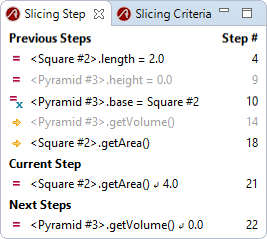
\includegraphics[width=0.50\textwidth]{img/slice1.png}
	\caption{The slice navigator view, for the program halted at \linerefn{lst:example}{6}.}
	\label{fig:slice1}
\end{figure}

Using this event list, the developer can obtain different kinds of information about the current state of the execution.
Firstly, simply by looking at the previous and next steps, the developer can understand at a glace how the current instruction fits into the grander scheme.
This is particularly useful if the current instruction was reached via a breakpoint, in which case it is not always obvious at which point in time it was hit.
To obtain this kind of information with a regular debugger, the developer needs to analyze the execution stack and maybe even inspect lower stack frames.

Secondly, it provides a summary of the program state.
Unlike a typical debugger's variable view, the slice navigator only shows relevant variables, and also shows relevant object fields on the first level.
Furthermore, the developer can easily investigate the origin of a value.
Simply clicking an event moves the execution to that point in time.
This way, the slice navigator allows to efficiently follow infection chains of erroneous state.

Thirdly, the slice navigator shows details about the dependency graph that was used to compute the current slice.
Small icons indicate how the events of the slice are related.
The next section explains how again the navigator serves not only as a visualization, but also allows the developer to interact with the underlying tools.

\subsection{Interactive Slice Configuration}

%When building the dependency graph between events, the algorithm distinguishes between three types of dependencies.
%\emph{Value dependencies} occur when the the value of an instruction is derived from another instruction's value.
%In the slice navigator, they are represented with a red equality sign.
%Instructions that determine if another instruction can be reached are \emph{reachability dependencies}, indicated by a yellow arrow.
%Typically, these are method invocations and instruction in conditional statements.
%Sometimes, a value depends on only one of multiple candidate values. 
%A \emph{control dependency} determines which of these candidates is used.
%More formally, control dependencies are reachability dependencies of value candidates that are not also reachability dependencies of all other candidates.
%In the navigator, they are indicated by a blue "X".

The developer can now combine these different dependency types to adjust the slice for specific purposes.
Clicking on an event's dependency symbol brings up a dialog that allows to choose which dependencies of that event to include.
This way the developer can, for instance, put a focus on how a value was computed or how an instruction was reached.
It is also possible to remove all dependencies of an event, for instance if it is known to be correct and its history is not of interest, thereby moving the focus of the slice to less well-understood parts of the program.

\begin{figure}
	\centering
		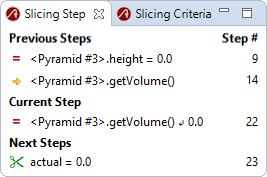
\includegraphics[width=0.50\textwidth]{img/slice2.png}
	\caption{The slice navigator view, for the program halted at \linerefn{lst:example}{6}.}
	\label{fig:slice2}
\end{figure}

Whenever a slicing criterion is modified, the slice is updated instantly, without locking the user interface or resetting the current debug session.
In our examples, the developer might choose to exclude the result of ´getArea()´ from the slice. 
As shown in \cref{fig:slice2}, with the computation of the area removed from the slice it is now much easier to see that the wrong result of ´getVolume()´ was caused by a wrong value in ´height´.


As mentioned before, instructions and states not belonging to the slice are still shown in the IDE, mostly to serve as an orientation help, to provide context to the current operations.
However, it might also happen that a value or instruction outside of the slice catches the developers attention.
In this case, she can choose to add it as another slicing criterion and the slice is immediately expanded.
Again, this happens without interrupting the developer's work.
In the worst case, expanding the slice takes as long as creating a new slice for only that event.
The developer might notice how new events are added to the slice in the background.
Generally, this should not be an impediment, as events that are closest to the current instruction are added first.

\subsection{Comparison with other Slicing Tools}


Compared to existing Java dynamic slicers, our approach has several advantages.
Unlike JSlice, we separated the tracing and the analysis phase.
This allows for faster results when computing multiple slices on the same execution.
Both JSlice and JavaSlicer allow to visualize the slice by highlighting relevant lines in the source code.
Our approach uses the slice in the context of a debug session, which means it not only allows to step through the slice, but also allows the developer to inspect variables and objects at any point in time.
Furthermore, the developer can choose to exclude different types of dependencies from a slice to set a focus, for instance, on calculation or reachability questions.

\begin{figure}
\centering
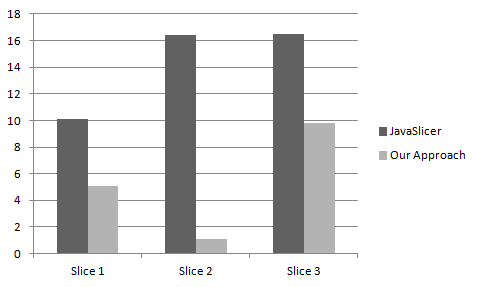
\includegraphics[width=.9\linewidth]{img/eval}
\caption{Total slicing time in seconds. Slice 1 is the example as introduced in Section 3, Slice 2 and 3 are derived from the same test-case with a different slicing criterion.}
\label{fig:eval}
\end{figure}

\autoref{fig:eval} shows the results of a preliminary performance evaluation, run on a 2.0 GHz Intel i7 Processor.
JSlice was not included in the experiments as it only supports older versions of Java.

For the example shown in this paper, our approach creates the slice in about 5 seconds and performs better than JavaSlicer.
Slice 2 and 3 were created from a test-case with longer runtime. 
For slice 2, the slicing criterion was chosen to produce a very small slice, while for slice 3 a larger slice from the same execution was created.
As the results indicate, the runtime of our approach grows linear with the size of the slice, while JavaSlicer's runtime appears to grow linear with the size of the whole trace.

Not shown in the diagram is that for every slice, about 70\% of the time was spend with static dependency analysis.
The results of this analysis can be cached to improve the responsiveness when different slices on the same methods are created.
Furthermore, our approach can be optimized for multi-threading, as both the static analysis of a method and the dependency resolution for an event are atomic operations that allow for high concurrency.

\section{Debugging in Database Applications}
%Concepts of Java solution apply to all structured imperative languages.\\
%SQLScript is one very important language that is different\\
%
%\subsection{Challenges in the New Domain}
%
%first, large amounts of data are challenge for tracer\\
%second, declarative elements\\
%we can use the latter to solve the former.
%
%\subsection{Modified Tracing in SQLScript}
%
%don't trace SQL, try to reproduce instead\\
%How ODB can be build from that\\

Many large and complex applications use a database to persist large amounts of data. 
However, with the advance of in-memory databases and the decline of RAM cost, the database is no longer seen as a simple data provider~\cite{plattner2011memory}.
For maximum performance, more and more business logic is moved away from the so-called application layer, which is typically coded in some high-level object-oriented language, into the database, where it has to be rewritten in SQL queries and stored procedures (mostly SQLScript).
The increasing complexity of database routines brings an increased need for tool support for debugging.

Regular debuggers for stored procedures already exist.
They allow to set breakpoints and to inspect variables and tables, as one would expect.
However, often they can not be used as efficiently as debuggers for other languages.
It is common for a stored procedure to run several seconds or even minutes, which increases the cost for restarting a debug session.
Furthermore, the large amounts of data that can be processed in a single call can make it impossible for the developer to gain a complete understanding of the program state.

Both problems can be solved by testing with minimal example data.
However, if the nature of a bug is not yet known, creating such an example may be impossible.
In this section, we show how an omniscient debugger for stored procedures can be realized and discuss specific problems such a debugger has to face.
A prototypical implementation is currently being developed.

\subsection{Tracing and Omniscient Debugging}

An omniscient debugger also suffers from the large amounts of data.
Our Java debugger traces every field and variable access.
Tracing every tuple of a table would create a dramatic overhead.
Using an even-bigger database, just to manage a single debug session, is not feasible.
Instead, we take advantage of the same that makes stored procedures so powerful in the first place: the declarative nature of SQL queries.

Unlike in object-oriented programs, where almost every behavior can be changed by virtual method calls, it is not possible to change the behavior of a where-clause.
Furthermore, SQL queries are well defined so that it is not necessary to analyze the internal workings to allow an analysis of the overall behavior.

Instead, we only need to trace variable assignments to be able to reproduce the program execution.
Queries don't have to be traced at all, although for some purposes it will be helpful to record some meta information, such as the execution time or the number of results.
However, we need to be able to reproduce the query results, otherwise the debugger would be quite useless.

\subsection{Reproducing Queries}

By tracing all variables, the debugger has enough information available to re-execute any query.
However, the query will only yield the same results as long as the underlying data has not changed.

In general, one can expect that debugging will take place on a development machine where no other data manipulation occurs.
However, in cases where this assumption doesn't hold, the debugger might end up showing wrong or misleading data the developer, which can make the tool outright harmful.
Furthermore, the debugged stored procedure itself may change the data, which will cause a query to return different results at different points in time.

We have identified three strategies of dealing with data changes, each with its own advantages and disadvantages.

\paragraph{Temporary Tables}
Auxiliary tables can be used to track all data changes.
Values of deleted tuples and modified attributes have to be recorded, as well as timestamps of the manipulation events.
To re-execute a query, it has to be rewritten to include this additional data.

An advantage of this approach is that it allows to efficiently analyze the modifications that were applied by the stored procedure.
Disadvantages are that copying data to auxiliary tables greatly increases the tracing overhead, and that rewritten queries are much more complex and thus may take longer to execute.

\paragraph{Transactions}
If the whole debug session runs in a single database transaction, it is automatically protected from concurrent modifications.
Nested transactions can be used to rollback changes done by the debugged code.

This approach requires only little effort by the debugger, as it builds upon existing features of the database.
However, to re-execute a single query, the whole stored procedure has to be re-executed up until that point, which can create a significant overhead.
Furthermore, depending on how transactions are implemented, the developer might accidentally lock the database for everyone else.

\paragraph{Insert-Only}
In systems that are relevant to accounting, such as ERP, finance, and CRM systems, data is never deleted.
Such behavior often even is a legal requirement.
If we require for all tables that data can never be changed or deleted and annotate all tuples with timestamps of when they have been created and invalidated, we can reconstruct the state of the database of any point in time.

This approach combines the advantages of both previous approaches.
Especially in in-memory databases, the overhead can be less than expected due to compression, and it may even improve the performance as inserts can be faster than updates or deletes.
Finally, adding timestamp filters to select queries does not cause a significant slowdown.

\subsection{Slicing}

The slicing algorithm that we presented in \cref{sec:slicing-algorithm} can be easily transferred to stored procedures.
Statements depend on each other through the variables they access, and from the variable trace the execution path that is necessary for dynamic slicing can be reconstructed easily.

However, the power of dynamic slicing comes from knowing where fields of objects are read and written.
In stored procedures, we would expect that the slicing algorithm can tell us which tuples of a table are actually relevant for the slice.
However, without tracing access to tables, this information is not immediately available.

\paragraph{Exact approach}

One way to find relevant tuples is to reproduce the filter expressions that were used to access a table.
By or-chaining all expressions, the result is the union of all individual query results.
Additional attributes can be introduced that indicate which of the filter expression matched for a tuple.
While this approach might not scale well when nested queries are involved, we are now, at least in principle, able to get a view on the database that reflects ours slice.

However, the slicing algorithm does not yet consider this information when computing a slice.
It might be the case that a particular filter expression, or a particular variable in a filter expression, does not affect the result set.
In this case, the expression or variable should be excluded from the slice.

In principle, it is possible to use this information when constructing a slice.
However, actually executing these queries can increase the time required for building a slice until it is no longer desirable. 

\paragraph{Approximate approach}

Another way to build a data slice is to approximate a filter.
Bloom filters use hashing to store subsets of large data in comparatively small bitmaps, at the cost of creating some false positives \cite{Pagh:2005:OBF:1070432.1070548}.
Inserting bloom filters at selected parts in the stored procedure can reduce the need to analyze larger parts of code and simplify filters that are used to compute slices.

\medskip

\noindent
A usable dynamic slicing algorithm could first create a slice without inspecting the tables.
In cases where more precision is needed, the developer could then choose to apply one of the approaches outlined above to refine the results.

\subsection{Time-travel Queries}

\lstMakeShortInline[basicstyle=\ttfamily,language={Inline},breaklines=true]`

In our set-up, the debugger trying to recreate intermediate results of a stored procedure is just a special use case for the ability to submit arbitrary queries against the database of any previous point in time.

The query shown in \cref{lst:ttravel} selects the total of open orders for previously selected projects.
We will use it as an example to demonstrate how \emph{time-traveling} queries are handled by our system.

\begin{lstlisting}[language=HanaSQL,float,caption={Example for a time-travel query: Select the current total of open orders for previously selected projects},label=lst:ttravel]
  SELECT pr.id, pr.name, pr.budget, SUM(po.total)
  FROM :selected_projects pr
	JOIN PurchaseOrders po ON po.project_id = pr.id
	WHERE po.status = 'open'
	GROUP BY pr.id, pr.name, pr.budget
	^§AT STEP§ 1623^
\end{lstlisting}

The last line shows an extension to SQL that can be used by the developer to explicitly query a point in time, with `^1623^` being an instruction ID that was obtained from the debugger UI.
If omitted, the current step can be derived from the context from which the query is submitted, such as an SQL console that is associated with a specific point in time or the current debug step.
The parameter `:selected_projects` refers to a variable from the current debug session and will be populated with its current value, independently of the value of the step-clause.

When submitted, our debugger applies two changes to the query before it can be submitted to the database.
First, all parameters are replaced with corresponding views.
When a stored procedure is debugged for the first time, the debugger automatically creates a view for each query in the procedure.
These views are identified by the target variable name and the line number and expect a step identifier and all parameters that the actual query takes.
In our example, `:selected_projects` might be replaced with `VAR_selected_projects_7(1055, 'Research')` when it was last set at step 1055 in code line 7 and called with the respective argument.

Second, a time-stamp filter is added for all tables that are referenced in the query. 
In our example, `po.createdOn < ^1623^ AND (pr.validTo IS NULL OR pr.validTo > ^1623^)` would be added to the Where-clause.

Now, the query can be submitted to the database and the result is subsequently presented to the user.

\subsubsection{Time-diff Queries}

To get a better overview about what happened in a piece of code, the developer might want to query multiple points in time at once and see the difference in the query result.
For this example, she debugs a stored procedure that processes the payments for projects, but sometimes allows projects to go over budget.
By stepping into the procedure, she has three defined points in time: `^before^`, at the beginning of the procedure; `^now^`, at the current instruction; and `^after^`, at the end of the execution.

Now she wants to compose a query that selects all projects that will go over budget and the orders that were processed.
The query is shown in \cref{lst:tdiff}.
\begin{lstlisting}[language=HanaSQL,float=b,caption={Example of a time-diff query: "Select all projects that will go over budget and their respective purchase orders"},label=lst:tdiff]
	SELECT pr.id, pr.name, pr.budget, SUM(po.total), po2.id, po2.status, po2.total
	FROM :selectedProjects pr
	JOIN PurchaseOrders po ON po.project_id = pr.id
	JOIN PurchaseOrders po2 ON po2.project_id = pr.id
	WHERE po.status = 'open'
		AND now!pr.budget > 0 AND after!pr.budget < 0
		AND before!po2.status != after!po2.status
	GROUP BY pr.id, pr.name, pr.budget, po2.id, po2.status, po2.total
	^§AT STEP§ before=817, now=1623, after=2043^
\end{lstlisting}
Like before, the `^AT STEP^` clause does not have to be explicitly typed in the query, but can also be derived from the context.
A language extension allows to add filter conditions that only apply to specific points in time.
\Cref{tab:diffresult} shows a possible result for this query, with one project that goes over budget and two associated purchases, of which one was already processed.

\newcommand{\red}[1]{\textcolor{DarkRed}{#1}}
\newcommand{\gr}[1]{\textcolor{Green}{#1}}

\ctable[caption={Result of a time-diff query, with multiple values in some columns},label=tab:diffresult,doinside={}]
				{rlrrrlr}{}{
	pr.id & pr.name 	& pr.budget & total & po2.id & po2.status & po2.total \ML
	
				&					 & \red{1200} & \red{1500} &	 & \red{open} &						\NN
	1			& Project 1 & 200				& 500 			 & 1 & paid 			& 1000			\NN
				&						& \gr{-300} & \gr{0}		 &	 &						&						\ML

				&					 & \red{1200} & \red{1500} &	 & 						&						\NN
	1			& Project 1 & 200				& 500 			 & 2 & open 			& 500				\NN
				&						& \gr{-300} & \gr{0}		 &	 & \gr{paid}	&						\ML
}

To produce this result, the query has to be executed three times, once for each point in time, without the time-specific filter conditions.
Then, to prepare the diffing of the results, they are outer-joined on the primary keys and the time-specific filters are applied.
For performance reasons, all of this happens inside a single SQL query, as shown in \cref{lst:tdifffinal}.
The execution of the sub-queries is indicated in \linerefn{lst:tdifffinal}{6, 7, and 10}, the time-specific filters can be found in the Where-condition of \linerefn{lst:tdifffinal}{15 and 16}.

\begin{lstlisting}[language=HanaSQL,float,caption={Parts of the time-diff query after transformation},label=lst:tdifffinal]
	SELECT COALESCE(__before."pr.id", ...) AS "pr.id",
	       COALESCE(__before."po.id", ...) AS "po.id",
				 __before.createdOn as _step_0,
				 __before."pr_name" AS "pr_name_0", ...,
				 ...
	FROM (SELECT ... ^§AT STEP§ before^) __before
	FULL OUTER JOIN (SELECT ... ^§AT STEP§ now^) __now
	    ON __before."pr.id" = __now."pr.id" 
		 AND __before."po.id" = __now."po.id"
	FULL OUTER JOIN (SELECT ... ^§AT STEP§ after^) __after
	    ON (__before."pr.id" = __after."pr.id" 
		      AND __before."po.id" = __after."po.id")
		  OR (__now."pr.id" = __after."pr.id" 
		      AND __now."po.id" = __after."po.id")
	WHERE __now."pr.budget" > 0 AND __after."pr.budget" < 0
	  AND __before."po.status" != __after."po.status"
\end{lstlisting}

For the final result, the key attributes are coalesced while the other attributes are selected from each point in time.
Furthermore, for each tuple its creation step is selected.
This value is needed for two reasons: first, it is necessary to distinguish between tuples with `NULL` values and tuples completely missing from the result; second, it allows the debugger to know when the value was created or changed.

In the UI, the before and after values are only shown if they differ from the now value.
Clicking on value allows the developer to jump to the `UPDATE` or `INSERT` statement that caused the change.

\subsubsection{Limitations}

Currently, our approach has two major limitations.

First, time-diff queries can only be executed on tables that have clearly defined primary keys, for key attributes are required to track a tuple's versions over time.
For a query like "Sum budgets per project category", it has to be clear that categories are the entities that keep their identity over time.
Here, an additional syntax extension could be used to convey this kind of information.

Second, it is currently not possible to use time qualifiers outside of the `WHERE` clause.


\subsection{Dynamic Slicing on Large Amounts of Data}

Object centric/Data centric debugging: Problem of opaque tables\\
Comparison of data governance approaches.\\
Our slicing algorithm for SQLScript. Interactive approach to improve slice quality on demand\\

\section{Evaluation}

Summary of technical evaluations.\\
todo: let some people try it, stop the time

\section{Conclusion and Future Work}

\nocite{*}
\renewbibmacro{in:}{}
\printbibliography[]

\end{document}
